Let $n\geq 2$. We begin this section by reviewing the definition of the Burau representation 
\[\Psi_n : B_n \to \mathrm{GL}_{n-1}(\mathbb{Z}[t^{\pm1}]).\] Then we discuss the criterion for faithfulness introduced by Moody and refined by Long--Paton and Bigelow.

\subsection{Burau via braids acting on cyclic covers}

One incarnation of the braid group $B_n$ is as the mapping class group of $D_n$ \cite{Bir74}, the disk with $n$ marked points in its interior, as depicted in Figure~\ref{disk} for $n=4$. Viewing the marked points as punctures, the fundamental group of $D_n$ is the free group $F_n$. With $p_0$ a basepoint on the boundary, a free basis is given by $X := \{ x_1, \dots , x_n \}$, where $x_i$ is the loop traveling around $p_i$ in the clockwise direction.

\begin{figure}[h]
\begin{center}
\begin{overpic}[width=2.7in]{disk.png}
\put(48,7){$p_0$}
\put(19,43){$p_1$}
\put(39,43){$p_2$}
\put(58,43){$p_3$}
\put(78,43){$p_4$}
\put(29,55){$\alpha$}
\put(68,55){$\beta$}
\end{overpic}
\caption{The $4$-punctured disk, $D_4$. Straight line arcs $\alpha$ and $\beta$ are depicted.}
\label{disk}
\end{center}
\end{figure}

Consider the cyclic cover $\tilde D_n$ of $D_n$ associated with the kernel of the exponent sum map $F_n = \langle X \rangle \to \Z$. This cover is formed by taking a copy or `level' of $D_n$ for each integer, cutting along a straight-line arc from the boundary to each puncture in every level, and then gluing appropriately. The cover $\tilde D_n$ has the structure of a free $\mathbb{Z}[t^{\pm1}]$-module endowed upon its first (integral) homology group, with $t$ corresponding to a choice of generator of the cover's deck group, $\Z$. The action of $B_n$ on $D_n$ preserves the kernel of the exponent sum map, and thus lifts to $\tilde D_n$. The free $\mathbb{Z}[t^{\pm1}]$-module $H_1(\tilde D_n)$ has rank $n-1$, and the \emph{(reduced) Burau representation} $\Psi_n : B_n \to \mathrm{GL}_{n-1}(\mathbb{Z}[t^{\pm1}])$ assigns to each braid the $\Z[t^{\pm 1}]$-linear transformation of $H_1(\tilde D_n) \cong \mathbb{Z}[t^{\pm1}] ^ {(n-1)}$ that it induces.

\subsection{A criterion for faithfulness}

An \emph{arc of type $(i,j)$} in $D_n$ is the (oriented) image of a continuous embedding of the unit interval $[0,1]$ into $D_n$, whose endpoints are $p_i$ and $p_j$. Given arcs $\alpha$ and $\beta$ of some (perhaps distinct) type, the \emph{Burau polynomial} \cite{LP93} is defined to be
\[ \int_{\beta} \alpha := \sum_{j \in \mathbb{Z}} \hat \iota (t^j \cdot \tilde \alpha , \tilde \beta) t^j ,\] where $\tilde \alpha$ and $\tilde \beta$ are some choice of lifts of $\alpha$ and $\beta$ respectively, and $\hat \iota$ denotes algebraic intersection in $\tilde D_n$. Note that this polynomial is only well-defined up to multiplication by $t$, and that $\int_{\beta} \alpha$ and $\int_{\alpha} \beta$ are obtained from each other by replacing $t$ by $t^{-1}$ and negating coefficients. For a comprehensive discussion of calculating Burau polynomials in practice, we refer to Bigelow \cite{Big99}.

The following criteria, written as appears in \cite{Big99}, allow us to use Burau polynomials to investigate the faithfulness of the Burau representation.

\begin{theorem}[Bigelow \cite{Big99}] \label{the:criterion}Let $n \geq 3$. The following are equivalent:
\begin{enumerate}\item The Burau representation $\Psi_n$ is unfaithful.
\item There exist essentially intersecting arcs $\alpha$ and $\beta$ in $D_n$ of types $(1,2)$ and $(3,4)$ respectively, with zero Burau polynomial.
\item There exist essentially intersecting arcs $\alpha$ and $\beta$ in $D_n$ of types $(1,2)$ and $(0,3)$ respectively, with zero Burau polynomial. 
\end{enumerate}
\end{theorem}
The proof of Theorem~\ref{the:criterion} is given in Bigelow. While it does not explicitly show that the second statement implies the third, this may be established using techniques similar to those found elsewhere in the proof.

Variants of these criteria for faithfulness have been used to show that $\Psi_n$ is not faithful for large $n$. Moody \cite{Moo91} initially obtained a lack of faithfulness for $n \geq 9$, which was improved to $n \geq 6$ by Long--Paton \cite{LP93}. Most recently, Bigelow \cite{Big99} showed that $\Psi_5$ was not faithful. The remaining case to investigate is $n = 4$; our goal for the remainder of the paper is to do so.

To close this section, we give a proof that the Burau polynomial of an arc-pair is invariant under the action of the braid group. We will use this fact repeatedly to simplify the calculations we carry out.

\begin{proposition}Let $\phi \in B_n$ for $n \geq 2$. Then for any arc $\alpha$ of type $(i,j)$ and $\beta$ of type $(k, l)$ in $D_n$, we have \label{preserve}
\[ \int_{\beta} \alpha = \int_{\phi \cdot \beta} \phi \cdot \alpha . \]
\end{proposition}
\begin{proof}
We check that the proposition holds when $\phi$ is one the standard half-twists generating the braid group $B_n$ (i.e. the half-twist $\sigma$ interchanging adjacent punctures seen in Figure \ref{halftwist}).

Given any arcs $\alpha$ and $\beta$, we may assume that any points of intersection between them lie outside of the support of $\sigma$, by either isotoping the arcs or the half-twist. Locally, $\alpha$ and $\beta$ can be taken to look as in Figure \ref{pre}, with, perhaps, the segment of the red curve beginning and ending in a different position relative to the punctures.

\begin{figure}
\centering
\begin{subfigure}[t]{0.4\textwidth}\centering
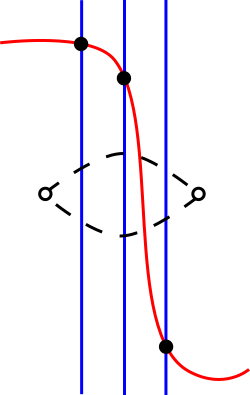
\includegraphics[width=1.6in]{preserve.png}  
\caption{The half-twist $\sigma$ is supported on a regular neighborhood of the two dashed arcs.}
\label{pre}
\end{subfigure}
\quad
\begin{subfigure}[t]{0.4\textwidth}\centering
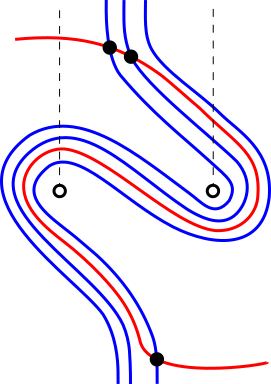
\includegraphics[width=2in]{preservepost.png} 
\caption{The dashed vertical lines indicate when the arcs' lifts change levels in the cover $\tilde D_n$.}
\label{post}
\end{subfigure}
\caption{The effect of $\sigma$ on the arc-pair $(\alpha, \beta)$. Subfigure (a) depicts a generic local picture of intersections between the pair. Subfigure (b) shows the result of applying $\sigma$.} \label{halftwist}
\end{figure}

When the half-twist $\sigma$ is carried out, the arc segments weave first around one puncture, then the other. Passing to the cover $\tilde D_n$, this corresponds to the arcs' lifts first climbing one level, traveling to the other puncture, then descending to the original level. Since no intersections between $\alpha$ and $\beta$ occur during this detour, it has no effect upon our calculation of the Burau polynomial of the pair. Thus, the half-twist $\sigma$ leaves the Burau polynomial unchanged.
\end{proof}
